\documentclass[]{article}

\usepackage{mathtools,mathrsfs,url,fancyhdr, graphicx,amssymb,amsthm,tensor,listings,float,color}
\usepackage[dvipsnames]{xcolor}
\graphicspath{ {images/} }

%opening
\title{Introduction into General Relativity\\Assignment 5.1\\Penrose--Carter diagram for an eternally accelerating observer/particle}
\author{Simon Crase}

\begin{document}

\maketitle

\section{Penrose--Carter diagram}

Figure \ref{fig:penrose-carter} depicts the Penrose-Carter Diagram, and Figure \ref{fig:minkowski} shows part of the World line in Minkowski space. The Minkowski diagram shows only a portion of the World Line, $s\in [-2,2]$, as otherwise it is impossible to distinguish the World Line from its asymptotes by eye. Both figures were generated by the Python program shown in Section \ref{section:source}.
\begin{itemize}
	\item It should be clear from \ref{fig:penrose-carter} that light rays from the constant-acceleration curve will eventually intersect $\cal{J}^+$.
	\item The figure includes a (dotted) line representing the World Line of a photon. Light from the constantly accelerating particle will intersect  $\cal{J}^+$ below the point where the photon's World Line intersects  $\cal{J}^+$.
	\item If the accelerating particle acts as an observer, its view of  $\cal{J}^-$ is restricted to the portion below and to the right of where the dotted line intersects $\cal{J}^-$.
\end{itemize}
\begin{figure}[H]
	\caption{Penrose-Carter Diagram for eternally accelerating observer/particle}
	\centering
	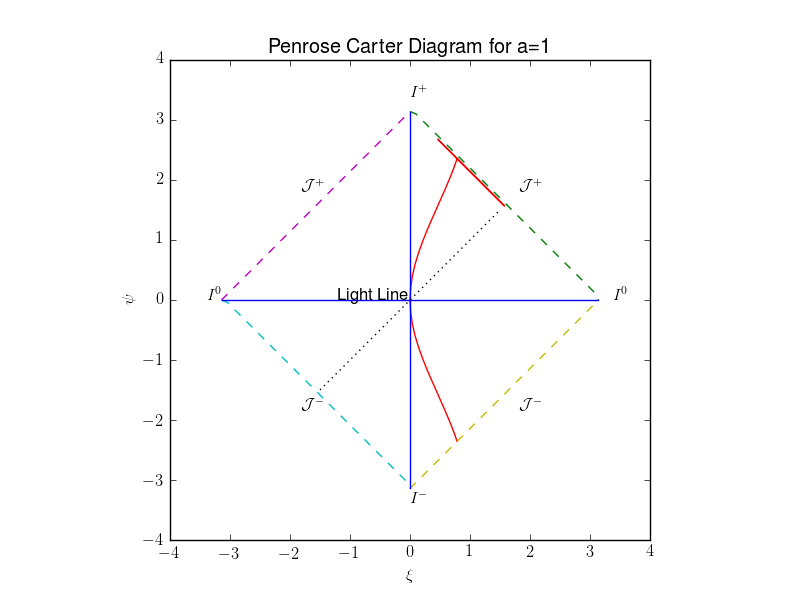
\includegraphics[width=1.0\textwidth]{GR-Problem-5-1-2.png}
	\label{fig:penrose-carter}
\end{figure}

\begin{figure}[H]
	\caption{Minkowski Diagram for eternally accelerating observer/particle}
	\centering
	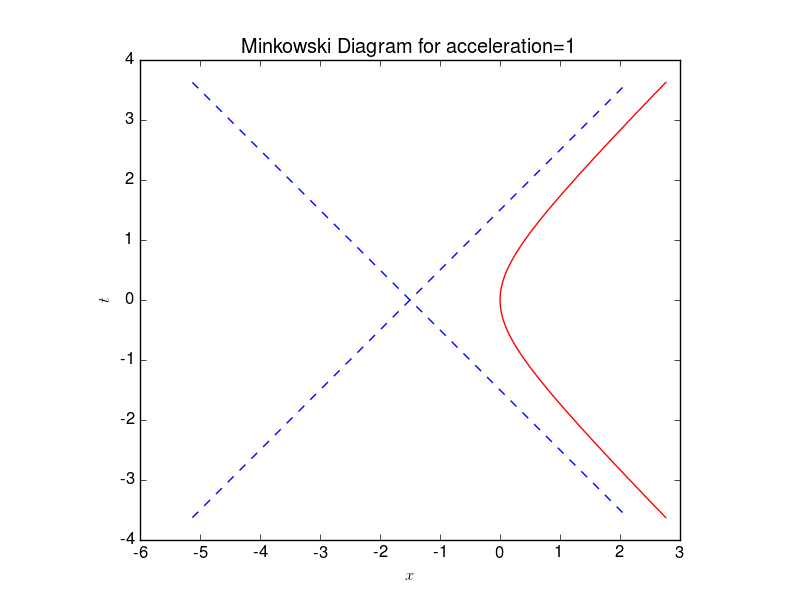
\includegraphics[width=1.0\textwidth]{GR-Problem-5-1-1.png}
	\label{fig:minkowski}
\end{figure}

\section{Python Source Code}\label{section:source}

Figures \ref{fig:penrose-carter} and \ref{fig:minkowski} were generated by the Python program which follows.
\lstinputlisting[language=python,frame=single,title=\lstname,backgroundcolor=\color{Apricot},breakatwhitespace=true,keywordstyle=\color{blue},commentstyle=\color{red},stringstyle=\color{Magenta}]{GR-Problem-5-1.py}

\begin{thebibliography}{9}
	
	\bibitem{akhmedev2016}
	Emil T. Akhmedev,
	\emph{Lectures on General Theory of Relativity},
	2016,
	\url{https://arxiv.org/pdf/1601.04996v6.pdf}.

\end{thebibliography}


\end{document}
